\documentclass[A4,openany,12pt]{article}
\usepackage{graphicx}
\usepackage{apacite}
\usepackage{amsmath}
\usepackage{float}
\usepackage{wrapfig}
\usepackage{lipsum}
\usepackage{setspace}
\usepackage{ragged2e}
\usepackage{tikz}
\usepackage{fancyhdr}
\usepackage{color}
\usepackage{natbib}
\usepackage[chapter]{algorithm}
\usepackage{pifont}
\usepackage{nomencl}
\makenomenclature

%\usepackage{charter}
\usepackage[bitstream-charter]{mathdesign}
\usepackage{parskip}
%\setlength{\parindent}{15pt}
\pagestyle{fancy}
\fancyhf{}
%\fancyhead[LE,RO]{\rightmark}
%\fancyhead[RE,LO]{\thepage}
%\fancyfoot[CE,CO]{\thepage}


\begin{document}
\onehalfspacing

\begin{titlepage}

\thispagestyle{empty}
\enlargethispage{1.3cm}

\vspace*{-1.9cm}
	

\includegraphics[width=\textwidth]{graphics/tex_dtu_uk_a1_cmyk.pdf}
	

\begin{raggedleft}
\vspace{\stretch{1}}

		
\Huge\textbf{Google Loon Project}\\[0.5cm]

\large{B.Sc.Thesis, June 10$^{th}$ 2016}\\[0.5cm]

\large \textbf{K\'ari Thrastarson, s131896}\\[1.5cm]		
\vspace{\stretch{1.8}}
\end{raggedleft}			
\begin{raggedright}
\large Supervisor: \\
\Large Jan Madsen\\ 
\large Professor in the Department Mathematics and Computer Science DTU
\end{raggedright}


\end{titlepage}
	

\tableofcontents 
\thispagestyle{empty}
\listoftables
\thispagestyle{empty}
\listoffigures
\thispagestyle{empty}
\printnomenclature
\thispagestyle{empty}
\cleardoublepage
\pagenumbering{arabic}


\addtocontents{toc}{\protect\thispagestyle{empty}}

\section{Introduction}
%Nowadays the Internet is no longer only a source of entertainment and leisurely activities, but an essential part of everyday operations. There should be no need to list all of the important roles this technology plays in people's everyday routine, but this list is actually getting longer every day. In light of these facts it is astounding to read the annual report from the \textit{Internet Society} which states that in 2013 60\% \citep{Brown} of the global population was still not able to connect to the Internet. 

The race has begun and many technology giants are now pursuing to hook the rest of the world up with an Internet connection for a reasonable price. But how can this be achieved? The companies each have their way of implementing this but they are all headed in the same general direction; up. They have all turned the usual way of communicating with an Internet provider upside down. As a person moved around he would connect with different radio towers, based on his current location. With the balloons this example is turned on its head. As the person stands still, he communicates with different balloons as they hover above and change location.

Whether the provider of the signal is a balloon, drone or some other device, the principal is the same. The technology has been strapped to a mobile object which moves around in the stratosphere and provides rural and remote ares with a 4G Internet connection. The aim of this project is to establish a foundation for a model that simulates the efforts being made by Google, but their team is focusing on balloons. The model will generalize the behaviour and simplify the universe to some extent. Reasoning for all assumptions will be provided as they are made. Rather than honing in on a perfect solution, several control algorithms are developed for the balloons  during this project and they aim to explore different aspects of the problem in question. Each algorithm is explained and tested, and thoughts given on its pitfalls and how they could be improved.

The data used is not actual weather data but randomly, but realistically, generated mock data. To further enhance the accuracy of the model actual stratospheric weather data could be used as an input.

\section{The loon project}
%\input{}

\section{The Model}\label{theModel}

\subsection{Introduction}\label{theModel_intro}
The loon project aims to launch thousands of balloons, each carrying expensive equipment and heavy, not to mention dangerous when falling freely. It would be foolish to attempt such a thing before making sure that the end goal is plausible, if not definitely possible. This can be done relatively cheaply using computer simulations, which is exactly the aim of this project.

The balloons are located in the stratosphere so they escape the winds and weather conditions that we experience from the troposphere. The balloons float with stratospheric currents that are more regular than the wind the troposphere and more predictable. The layers are multiple and differ between altitude. This means that the steering of the balloons is done simply by going up or going down. The balloons can decrease or increase their altitude to catch a new wind layer and go to another direction. 

Even though the world has been simplified significantly and many laws of physics overlooked, the simulation should give a good idea as to whether this idea is good or poor. Arguments are provided for all assumptions made during the modelling and their implications.  


\subsection{Description}\label{theModel_description}
The model focuses on the balloons and their movement around the stratosphere. The key components in the model are the following:

\begin{description}
    \item[The balloons:] The balloon travels around the stratosphere and supplies Internet connection to the point on the grid it corresponds to. 
    \item[The "grid":] The earth in this model is represented by a two dimensional array, or a grid, of integers. There are several, equally sized, grids that contain information about the status of the system. One holds the number of balloons hovering over current spot. Another grid is of type boolean and is computed based on the position of the balloons and it displays the coverage on the surface of the earth. True means connected, false means not. This is calculated using the position of the balloons and range parameter in the model. The goal is to fill this grid with as many true values as possible. 
    \item[The stratosphere:] The stratosphere is a collection of stratospheric wind layers which also are represented by a grid. The size of each wind layer equals the size of the earth grid. The layer object holds a collection of vectors which carry the wind strength in directions x and y. The stratosphere is organized so each wind layer occupies a certain altitude. That way each balloon is affected by only one wind layer at a time, determined by its current altitude. 
\end{description}

The model has some modifiable key parameters which are explained in chapter \ref{theModel_snp}. The model creates and initializes the ecosystem, which consists of the wind layers and the grid representing the earth. The simulation then starts populating the model with balloons, one during each iteration. The model then moves each balloon according to its corresponding wind layer. The decision a balloon has to make is whether it should start moving upwards, downwards or stay put. This decision is the core of the model and will be developed in different ways and compared.




\subsection{Data}\label{theModel_data}
The only data necessary for this simulation is stratospheric weather data. The blabla

\begin{figure}[h]
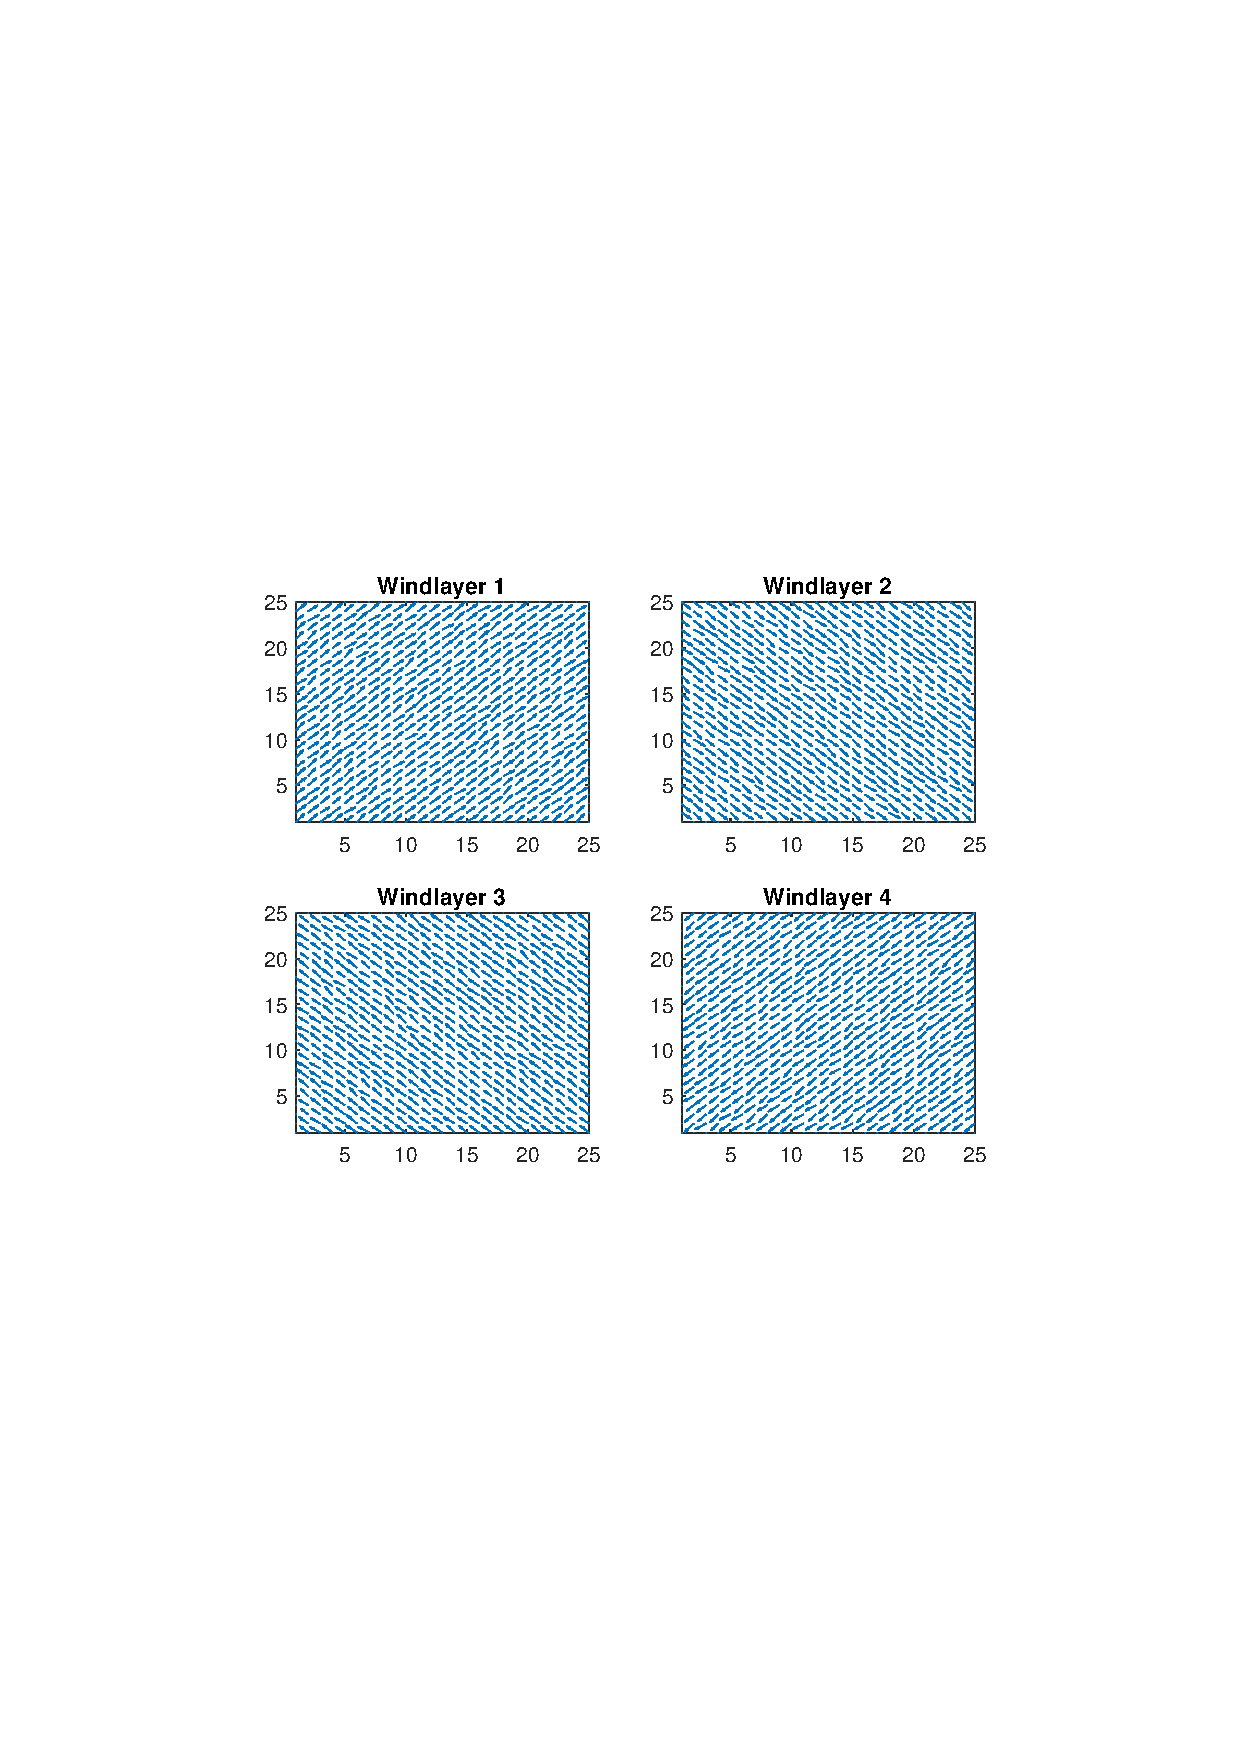
\includegraphics[trim={4cm 10cm 4cm 9cm},clip]{graphics/WindLayers.pdf}
\label{windlayers}
\caption{Wind Layers}
\end{figure}



\subsection{Simulation and Parameters}\label{theModel_snp}
The model is the structure and relationship between all objects. It is modifiable in some ways to be able to measure and compare performance of different algorithms. The parameters that should be adjusted before simulation are the following:

\begin{description}
\item[WORLD\_SIZE:] The integer dimension of the grid that represents the earth. This number greatly affects the run time of the model as well as accuracy. 
\item[NUMBER\_OF\_BALLOONS:] The number of balloons in the model. This variable is usually set to the number of cells in the earth grid, i.e WORLD\_SIZE$^2$.This means that best case scenario the coverage is 100\% and all the balloons are perfectly spread.
\item[VERTICAL\_SPEED:] The speed of the balloon in directions up and down. This number will be added/subtracted from the balloon's altitude each step, until its motion in that direction is stopped.
\item[NUMBER\_OF\_STEPS:] How many steps the simulation should run. This number should be as big as possible to properly model the behaviour of the ecosystem. 
\item[NUMBER\_OF\_CURRENTS:] The number of wind layers, or wind currents, in the system. The more layers there is to choose from the more accurate direction the balloon should be able to choose from.
\item[MIN/MAX\_ALTITUDE:] Numbers used to divide the layers. The total distance between MIN and MAX is divided equally between all the layers in the model. This is used to determine whether a balloon has reached a new wind layer. The units are abstract but should be taken into consideration when choosing vertical speed. The vertical speed corresponds to the units in this MIN/MAX scale.
\end{description}

The model and simulation go hand in hand. When all objects have been created and configured, the simulation is run. 

The simulation moves all balloons according to the established stratosphere. Each step of the simulation the following process is as follows:

\begin{enumerate}
    \item Apply decisions: All balloons decide, using the control algorithm, whether they should start moving up or down or stay in the current altitude. 
    \item Apply currents: When the decision has been made, all the balloons are moved according to the wind layer they are currently located in. Furthermore they are moved up or down according to the model parameter for vertical speed. 
    \item Update statistics: The statistics of the simulation are gathered on the fly so after each iteration the data is re-evaluated and stored for further analysis.
\end{enumerate}




\subsection{Assumptions}
%\input{}


\subsection{Measurements}
%\input{}

\subsection{Design}
%

This model was designed following the \textit{General Responsibility Assignment Software Patterns} (GRASP). The GRASP design principles provide guidelines for object-oriented software design and are well suited for a project such as this. The main focus of the principles, like the name states, is assigning responsibilities to the appropriate objects in the model. The basic roles in GRASP can be divided into \textit{knowing} and \textit{doing}. The design of the loon model is simple so the division was straight forward:
\begin{itemize}
\item[BALLOON:]
    \subitem Knows: A balloon object knows its own location, altitude and in which wind layer it is currently located.
    \subitem Does: A balloon object can move with the wind. It gets the wind vectors from the wind layer in which it is located. 

\item[WIND LAYER:]

    \subitem Knows: A wind layer object knows its own identification number, as well as the wind vector at any given place in the grid.
    \subitem Does: A wind layer does nothing but provide access to its data.

\item[WORLD:]

    \subitem Knows: The world know about the status of the simulation and how many steps have been taken. It collects statistical data about the grid in which the balloons hover. 
    \subitem Does: The world has access to all balloons and wind layers and is the controller of the simulation. The world initiates all decisions and movements of every balloon. 

\end{itemize}

The Balloon and WindLayer are expert classes while World is a controller class in this model. The algorithms developed during this project will be centralized, i.e controlled by an entity with knowledge of the entire system and access to all objects. This limits the balloons' responsibility to simply stay in the air, take commands and supply Internet coverage.

\begin{figure}[H]
    \centering
    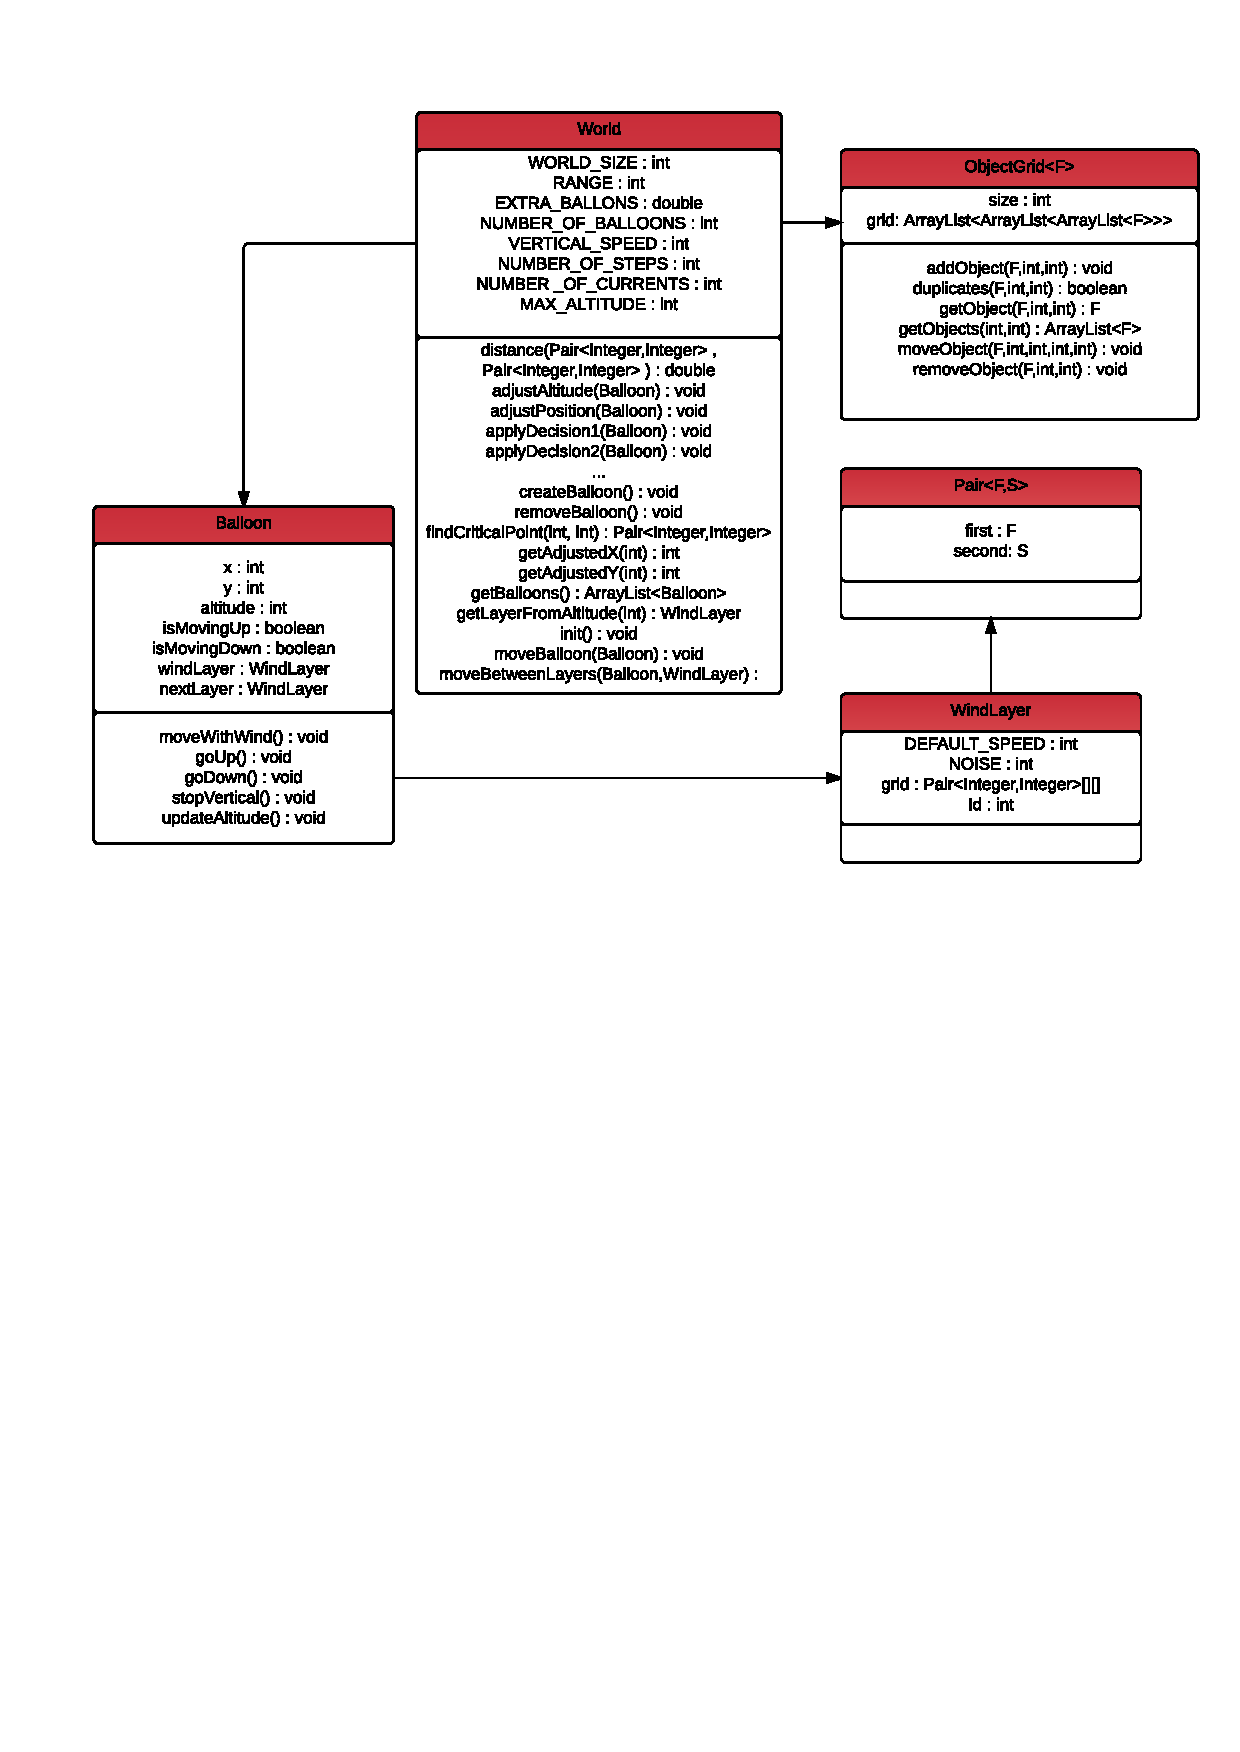
\includegraphics[width=\textwidth, trim= 1cm 14cm 0cm 0cm, clip]{graphics/classDiagram.pdf}
    \caption{Class Diagram}
    \label{fig:class_diagram}
\end{figure}


\begin{figure}[H]
    \centering
    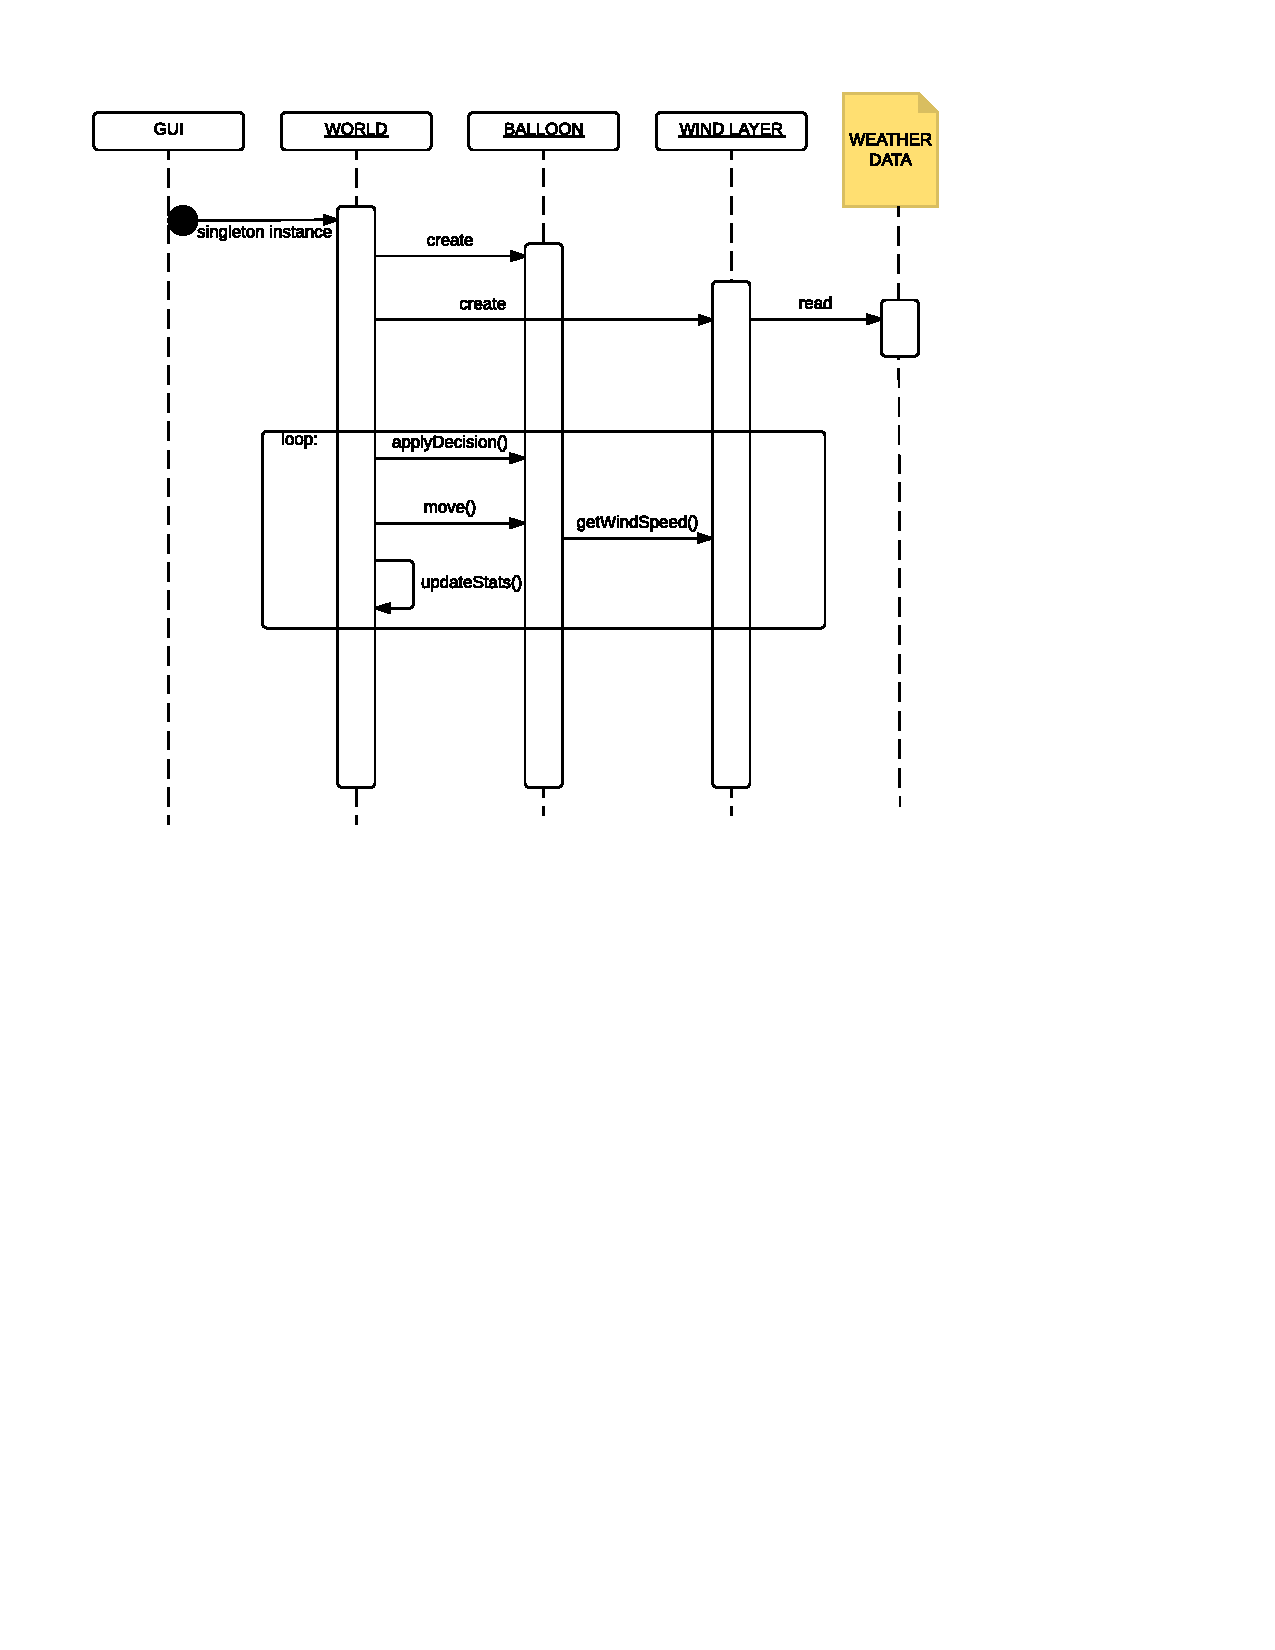
\includegraphics[width=\textwidth, trim= 1cm 12cm 4cm 1cm, clip]{graphics/sequenceDiagram.pdf}
    \caption{Simplified Sequence Diagram}
    \label{fig:seq_diagram}
\end{figure}



\subsection{Implementation}
%The programming language of choice for this project was JAVA. That was well suitable for an object oriented problem such as this. Eclipse was used as an IDE not only because of familiarity, but also due to all the handy refactoring tools that come built in to the environment. This is helpful when the code starts to look complicated, to be easily able to extract lines of code and store it within a private helper function. The toolkits SWING and AWT were used for the development of the GUI.

The project was stored on GitHub\footnote{www.github.com/karithrastarson} and is accessible to everyone. The process was iterative where a running version of the model was ready early, and then built upon for the duration of the period.
\subsection{Balloon}

The balloon class is an expert for the balloon. The following attributes are used to describe the object:
\begin{description}
	\item[int x]: X coordinates in the plane
	\item[int y]: Y coordinates in the plane
	\item[int altitude]: the altitude is used to determine wind layer
		\item[int age]: the number of steps this balloon object has taken.
	\item[boolean isMovingUp]: Used to determine whether this balloon is currently moving up.
	\item[boolean isMovingDown]:Used to determine whether this balloon is currently moving down.
	\item[WindLayer windLayer]: The current wind layer this balloon is located in.
	\item[WindLayer nextLayer]: Used to determine whether where this balloon is headed.
\end{description}

The balloon's main function and responsibility to the model is to move with the wind. This is done with the public function moveWithWind(). The balloon retrieves a wind vector from its current wind layer and adds the x and y components of that vector to its own current location in the grid. The new coordinates are then adjusted by the model, according to the border behaviour as described earlier. The adjustment is made as follows:

\begin{algorithm}[H]
\If{new x $\geq $ WORLD\_SIZE}{set x = x-WORLD\_SIZE}
\If{new x < 0}{set x = x+WORLD\_SIZE}

repeat for Y.\\
\end{algorithm}

The rest of the functions in the Balloon class are classic getters and setters, as well as a toString() and equals() functions.

\subsection{WindLayer}
The WindLayer class is an expert of weather data. Its main attribute is a grid of size equal to the WORLD\_SIZE global variable. The default constructor of the class takes two variables; an ID and the size of the world in which it will be. From that information the constructor takes care of generating mock data for the wind layer.

Two global variables are used to adjust the mock data:
\begin{itemize}
    \item DEFAULT\_SPEED = 45
    \item NOISE = 5
\end{itemize}

Algorithm \ref{alg:mockdata} displays how the mock data is generated. This model uses 4 layers and the constructor uses the ID to determine the general direction. The default speed variable is set to one of the four corners of the plane, based on the ID. Then a random number is generated on the scale from zero to the predefined max noise. Then a random boolean variable determines whether that random number should be added or subtracted from the x direction of the wind vector. Same routine is performed for the y direction. 

\begin{algorithm}[H]

\For {i from 0 to WORLD\_SIZE}{ 
    \For{j from 0 to WORLD\_SIZE}{


\If{Id=0}{x=DEFAULT\_SPEED and y=DEFAULT\_SPEED}


\If{Id=1}{x=DEFAULT\_SPEED and y=-DEFAULT\_SPEED}


\If{Id=2}{x=-DEFAULT\_SPEED and y=DEFAULT\_SPEED}


\If{Id=3}{-DEFAULT\_SPEED and y=-DEFAULT\_SPEED}

div = random number from 0 to NOISE

signX = random boolean

\If{signX}{x + div}
\Else{x - div}\endIf

div = random number from 0 to NOISE

signY = random boolean

\If{signY}{y + div}
\Else{y - div}\endIf

wind[i][j] = wind vector(x,y)
}
\EndFor}
\EndFor
\caption{Pseudocode for generating mock data}
\label{alg:mockdata}
\end{algorithm}


\subsection{Pair}
This class was created when a short survey on the Internet showed that JAVA was not equipped with a convenient generic container class that would store pairs, or tuples. It was easier to implement one from scratch. This class is really simple: it carries two variables of generic types T and R. Then the class is equipped with getters and setters. 

This class was created to contain the wind vectors. Each wind layer has a grid of Pairs. So a pair at coordinates x and y in a grid in the layer tells the wind speed and direction at that particular point.

\subsection{ObjectGrid}
No Java library had a suitable container for this project. The object that this project demanded was a two dimensional grid of a fixed size that could store zero or more objects in each cell. A generic class was implemented, but it was then utilized with Balloon objects in this particular project. This makes it easier to access a particular balloon object based on its coordinates.

The main container of the class looks complex but is in fact really simple. The class has the following attributes:

\begin{lstlisting}
    private ArrayList<ArrayList<ArrayList<F>>> grid;
    private int size;
\end{lstlisting}

The outer two array lists are initialized in the constructor, and a grid of empty array lists created. This grid has the dimensions size x size. Each cell in the grid holds an array list of a generic type that can be populated and modified easily. To find the number of balloons occupying a certain spot, the size of the array list at the corresponding cell in the grid is generated and returned.

\subsection{World}
The world is the controller of the model and contains all the balloons, wind layers and the control algorithms. The class contains a lot of attributes who's sole purpose is debugging and printing to to create graphs. Those attributes will be left out of this documentation. 

The World class has the attributes listed in section \ref{theModel_snp}. The class has two main containers that make up the model:

\begin{lstlisting}
	private ArrayList<WindLayer> stratosphere;
	private ArrayList<Balloon> balloons;

\end{lstlisting}

In addition, the class has three containers that support the decision making and the statistical overview of the simulation:
\begin{lstlisting}
	private ObjectGrid<Balloon> balloons_grid;
	private boolean[][] coverage;
	\end{lstlisting}
The ArrayList called \textit{stratosphere} holds all wind layers of the model in an order. The ArrayList called \textit{balloons} is a collection of all balloons created by the model. The boolean grid called coverage is updated in every step of the simulation with boolean values; true for covered and false for not covered. The ObjectGrid called balloons\_grid keeps track of the position of all balloons in the system.


\begin{algorithm}[H]
    Clear the grid.\\
    \ForAll{Balloon b in balloons}
    {center = Pair(b.getX(), b.getY())\\
        \For{int i = b.getX() - RANGE; i $<$ b.getX() + RANGE; i++}{
        \For{int j = b.getY() - RANGE; j $<$ b.getY() + RANGE; j++}{
        point = Pair(i,j)\\
        
        coverage[i][j] = inCircle(center, point)
        }
        }
    }
 \caption{Update Coverage}
 \label{alg:updateCoverage}
\end{algorithm}

The World class has a private function called updateCoverage() which is in charge of updating the boolean grid. This is described with algorithm \ref{alg:updateCoverage}. This function iterates through all the balloon in the system and inspects a rectangular area around the center of the balloon. This rectangle is visualized in figure \ref{fig:gridAssupmtions}. Each point in this area is passed through a function called inCircle, which applies the mathematical function for a circle to determine whether the point is within the coverage range or not. Either this points is within range or not. The sum of of all connected points is calculated and compared against the sum of the previous step. The difference in covered cells is interpreted as a dropped connection. If the connected cells er fewer than they were in the round before, that means that somebody has lost his Internet connection.

\begin{align}
    \left(x - a \right)^2 + \left( y - b \right)^2=r^2.\notag
\end{align}
where
\begin{align}\notag
     		x &= \text{x-coordinate}\\\notag
				y &= \text{y-coordinate}\\\notag
				a &= \text{x-coordinate of the center point}\\\notag
				b &= \text{y-coordinate of the center point}\\\notag
				r &= \text{radius (Range)}\notag
\end{align}


The constructor is short and only initializes the containers mentioned above without populating them. Then a more elaborate initialization function (called init(char c)) can be called with a character as an input, indicating which algorithm to use for the simulation. The \textit{init} function creates four wind layers and adds them to the stratosphere. Furthermore it outputs the windlayers to text files so they can be plotted and analyzed. The outcome is displayed in figure \ref{fig:windLayers}. 

One by one the balloons are created at placed at point (0,0) in the grid. Each step of the simulation adds on balloon and moves the rest. This will prevent the cell (0,0) from clogging on the first step.
The simluation is a repetition of the private function \textit{step()} and repeated as many times as the parameter of the model says. Each step is an execution of the following:

\begin{algorithm}[H]
\If{No. of balloons in system $<$ NUMBER\_OF\_BALLOONS}{createBalloon()}

\ForAll{balloons in system}{
applyDecision()
moveBalloon()
}

\ForAll{balloons in system}{
\If{Age of balloon $\geq$ LIFETIME}{removeBalloon()}
}

updateStatistics()
\end{algorithm}

The applyDecision() function is the actual control algorithm to which another section of this paper is dedicated. The moveBalloon() function is the thoughtful procedure of moving the balloon in the model and updating the appropriate containers. First the altitude is adjusted according to the vertical speed if the balloon is marked as moving up or down. Then a check is performed to see if the change in altitude affected the wind layer in which the balloon is. This is done with a function called \textit{getLayerFromAltitude} where each wind layer is assigned a certain space between the global variables that indicate the maximum and minimum altitude. The \textit{windLayer} attribute of the balloon is then updated and compared to the \textit{nextLayer} attribute to see if the vertical movement of the balloon should be stopped or not. 

When the balloon has been placed in the correct wind layer it can be moved around in the grid of balloons with the corresponding wind vector. The previous location as well as the new location of the balloons are updated in the grid to represent the actual movement. 

\subsection{Control Algorithms}
%\input{}

\subsubsection{Description}\label{description}
%\input{TeX_files/controlAlgorithms_description}

\subsubsection{Algorithm 1}
%The first algorithm is straightforward and rudimentary. After all the balloons are deployed on the starting point the following logic helps the balloons determine whether it should move or not:

\begin{algorithm}[H]
  \If{More than 1 balloon at current space AND balloon is not moving}{
 	\If{At bottom layer} 
 	{Go up}
 	\ElseIf{At top layer}  	
 	{Go Down}
 	\Else  	
 	{Choose direction at random}
 }
 \Else
 {Stay in current layer}
 \caption{Control Algorithm 1}
 \label{alg1}
\end{algorithm}

This algorithm has an obvious downside since as it contains an element of random, which is usually not helpful in a control algorithm. Nevertheless, it spreads the balloons pretty thoroughly around the grid relatively fast. The control over the grid is however limited, and this would not be a suitable solution if the end goal is to provide stable coverage.

This algorithm might however be utilized as a part of a larger more complex algorithm. At the beginner stages of the balloon's life cycle it could prove helpful to get the balloon out of that first wind layer and join the huddle.  

\subsubsection{Algorithm 2}
%This algorithm is a step towards a more complex control algorithm. Some minor logic replaces the random generator in the previous solution. 

\begin{algorithm}[H]
  \If{More than 1 balloon at current space}{
  Calculate projections\;
  
 	\If{optionUp < optionDown} 
 	{Go up}
 	\Else
 	{Go down}

 }
 \Else
 {Stay in current layer}
 \caption{Control Algorithm 2}
 \label{alg2}
\end{algorithm}

The balloon fetches the wind vectors from neighbouring wind layers and uses them to weigh its options. It computes the number of balloons occupying three different cells:
\begin{enumerate}
\item The cell to which the balloon's current wind layer will move it.
\item The cell to which the the wind layer above the balloon's current wind layer would move it.
\item The cell to which the the wind layer below the balloon's current wind layer would move it.
\end{enumerate}

The algorithm then determines which option has the cell with the lowest number of balloons and chooses that direction.
\begin{figure}
\centering

\includegraphics[scale=0.2]{graphics/todo.png}
\caption{Calculate projections}
\label{fig:projections}
\end{figure}

\begin{figure}
\centering
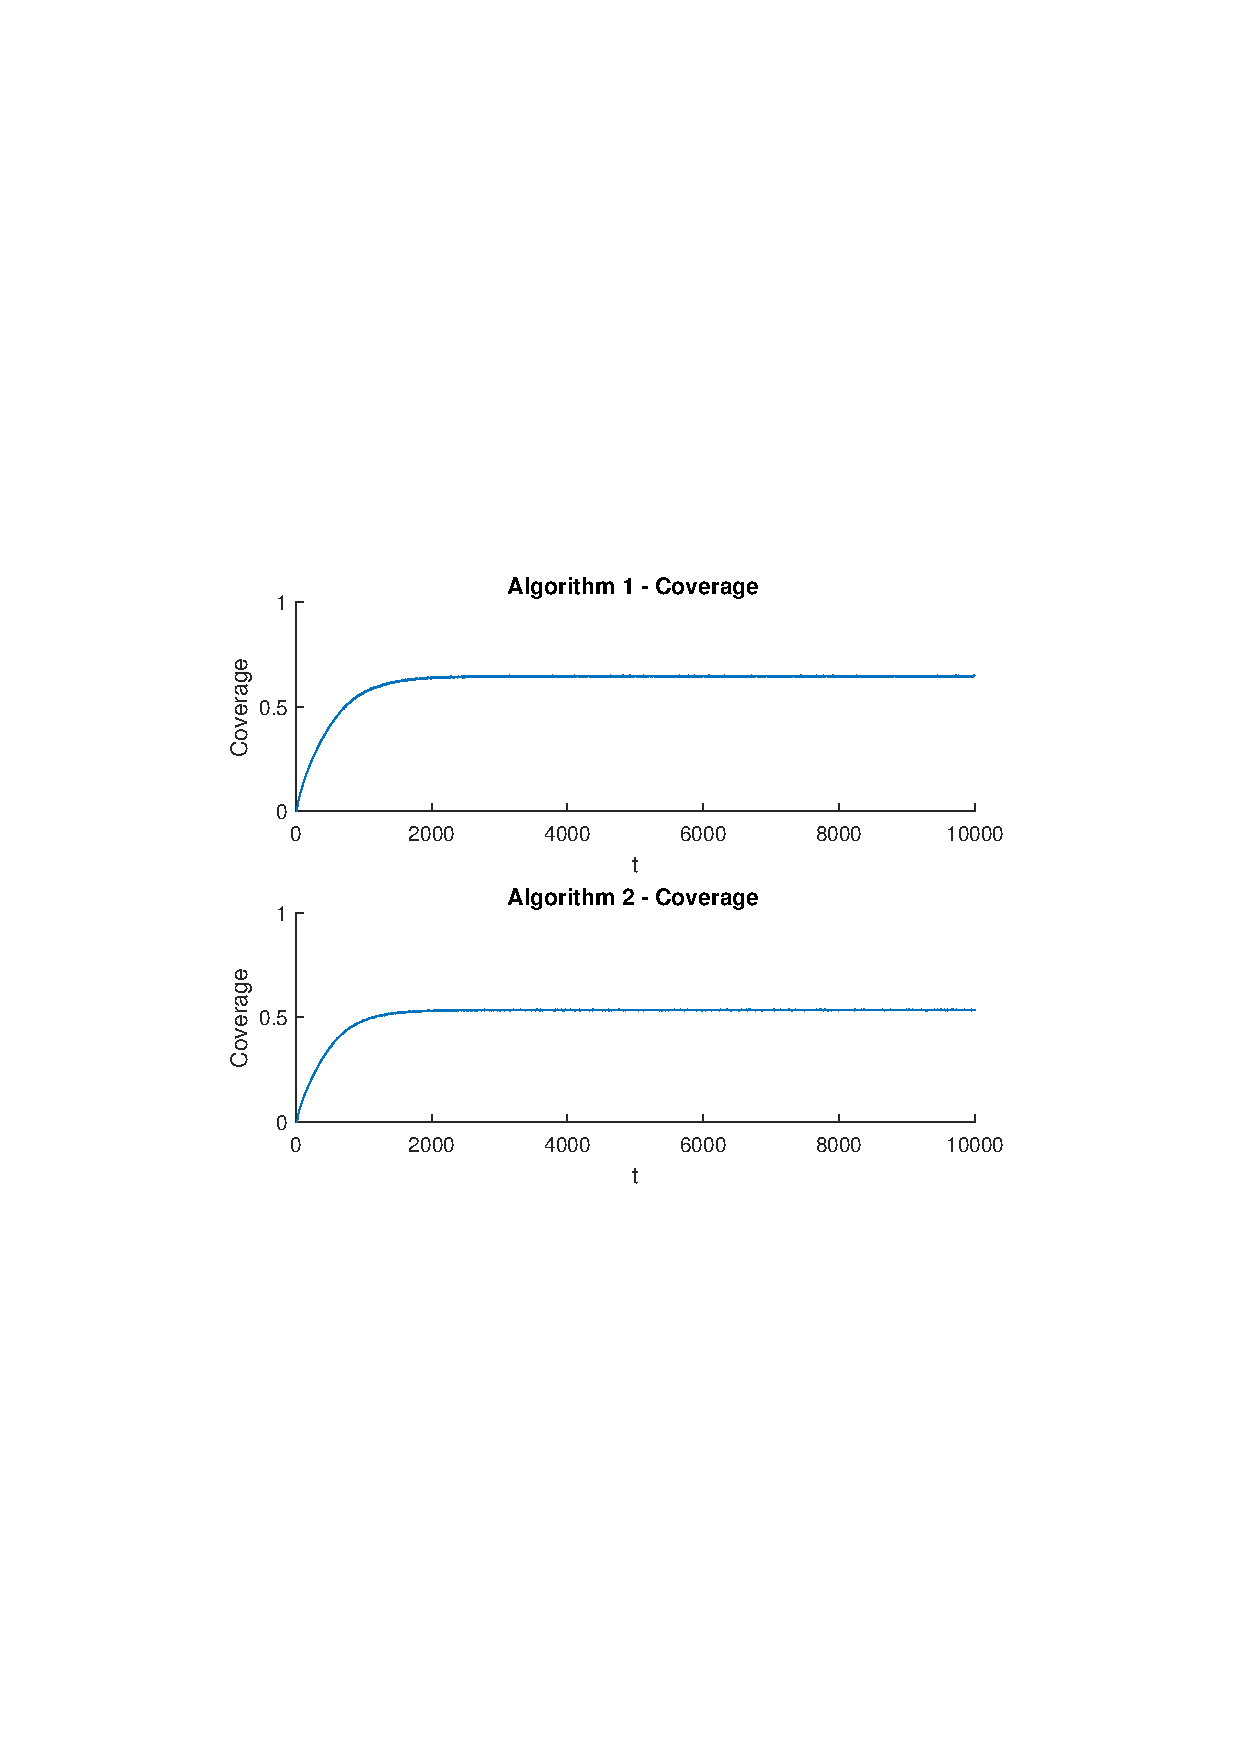
\includegraphics[width=\textwidth, trim={3cm 10cm 4cm 9cm},clip]{graphics/coverage_alg1_vs_alg2.pdf}
\caption{Algorithm 1 outperforms Algorithm 2}
\label{fig:alg1vsalg2}
\end{figure}
It is interesting to see that Algorithm 1 outperforms Algorithm 2 when it comes to coverage. Algorithm 1 reaches higher coverage like Figure \ref{fig:alg1vsalg2} clearly shows.

\subsubsection{Algorithm 3}
%\input{TeX_files/algorithm3}

\subsection{Comparison of performance and complexity}
%\input{}

\subsection{Data analysis of the simulations}
%\input{}

\subsection{Conclusion of simulations}
%\input{}

\section{Conclusion}
%\input{}

\printnomenclature
\nocite{*}
\bibliography{heimildir.bib}{} 
\bibliographystyle{apacite}

\end{document}